\documentclass[11pt,twocolumn]{article}

% Packages
\usepackage[utf8]{inputenc}
\usepackage{amsmath,amssymb,amsthm}
\usepackage{graphicx}
\usepackage{booktabs}
\usepackage{hyperref}
\usepackage{geometry}
\usepackage{natbib}
\usepackage{xcolor}
\usepackage{float}
\usepackage{caption}
\usepackage{subcaption}

% Geometry
\geometry{
    a4paper,
    left=2cm,
    right=2cm,
    top=2.5cm,
    bottom=2.5cm
}

% Hyperref setup
\hypersetup{
    colorlinks=true,
    linkcolor=blue,
    citecolor=blue,
    urlcolor=blue
}

% Custom commands
\newcommand{\Gini}{\text{Gini}}
\newcommand{\Tc}{T_{\text{c}}}
\newcommand{\vtest}{v_{\text{test}}}
\newcommand{\vobs}{v_{\text{obs}}}

% Title and authors
\title{\textbf{Scale-Invariant Information Coupling:\\
From Cosmic Velocities to Social Rigidity}}

\author{
    Johann Benjamin Römer$^{1,*}$ \\
    \small $^{1}$ Genesis Aeon Research Initiative \\
    \small $^{*}$ Corresponding author: \texttt{contact@genesisaeon.org}
}

\date{November 2025 \\ \small v5.0.0 - Empirical Grounding}

\begin{document}

\maketitle

\begin{abstract}
We investigate whether mathematical structures exhibit predictive correlations across disparate physical and social domains---a hypothesis we term \textit{structural isomorphism}. We test two specific predictions: (1) cosmic velocity scaling via fundamental constants ($\vtest = c/(\alpha^{-1} \cdot \Phi)$, where $\alpha$ is the fine-structure constant and $\Phi$ is the golden ratio), yielding $\vtest \approx 1352$ km/s vs. measured $\vobs = 1370 \pm 10$ km/s (1.3\% deviation, $p < 0.001$ vs. null model); (2) social phase transitions modeled via Ising dynamics with inequality as inverse temperature ($T_{\text{social}} = 1/(\Gini \cdot \text{Load})$), predicting critical transitions at high inequality. We calibrate model (2) against historical crisis data and perform Look-Elsewhere Effect scans for model (1) to quantify selection bias. Our findings demonstrate significant correlations but acknowledge critical limitations: post-hoc constant selection, $n=1$ cosmic system, and unverified causal mechanisms. We provide falsification criteria and transparent reporting of alternative models. This work offers a rigorous empirical test of cross-domain mathematical patterns while maintaining strict scientific skepticism.
\end{abstract}

\section{Introduction}

The search for universal patterns across disparate phenomena has driven scientific inquiry from Newton to modern complexity theory. However, claims of ``cosmic unity'' or ``universal laws'' often collapse under scrutiny when subjected to rigorous statistical testing and falsification criteria.

This paper tests a more modest hypothesis: \textit{do certain mathematical structures show predictive correlations across different domains?} We term this \textbf{structural isomorphism}---the hypothesis that similar mathematical frameworks (e.g., phase transitions, scaling laws) may provide predictive power in unrelated systems \textit{without implying causal connection or fundamental unity}.

\subsection{Two Testable Hypotheses}

We investigate two specific claims:

\paragraph{Hypothesis 1: Cosmic Velocity Scaling}
Can fundamental constants predict observed cosmic velocities? We test:
\begin{equation}
\vtest = \frac{c}{\alpha^{-1} \cdot \Phi}
\end{equation}
where $c$ is the speed of light, $\alpha \approx 1/137$ is the fine-structure constant, and $\Phi = (1+\sqrt{5})/2$ is the golden ratio. This yields $\vtest \approx 1352$ km/s, compared to the Bielefeld measurement \cite{boehme2021} of $\vobs = 1370 \pm 10$ km/s for solar system velocity through the CMB rest frame.

\paragraph{Hypothesis 2: Social Phase Transitions}
Can inequality-driven dynamics exhibit phase transition behavior analogous to physical systems? We model social adaptability using Ising dynamics:
\begin{equation}
T_{\text{social}} = \frac{1}{\Gini \cdot \text{Load}}
\end{equation}
where high inequality ($\Gini$) and cognitive/economic load reduce effective temperature, predicting transitions to ``frozen'' (low-adaptability) states.

\subsection{Critical Scientific Stance}

We emphasize:
\begin{itemize}
    \item \textbf{Correlation $\neq$ causation:} We report statistical patterns, not mechanisms.
    \item \textbf{Falsifiability:} All predictions include null hypothesis tests and alternative models.
    \item \textbf{Transparency:} We disclose limitations (post-hoc selection, small samples, unverified assumptions).
    \item \textbf{Look-Elsewhere Effect:} We quantify selection bias via systematic constant scans.
\end{itemize}

\section{Methods}

\subsection{Cosmic Velocity Hypothesis}

\subsubsection{Prediction}
Using CODATA 2018 values \cite{codata2018}, we compute:
\begin{align}
c &= 299\,792.458 \text{ km/s (exact)} \\
\alpha &= 7.2973525693 \times 10^{-3} \\
\Phi &= 1.618033988749895 \\
\vtest &= \frac{299\,792.458}{137.036 \times 1.618} \approx 1352.3 \text{ km/s}
\end{align}

\subsubsection{Null Hypothesis Testing}
We test against random constant pairs: generate 10,000 random dimensionless constants $c_1, c_2 \in [0.001, 0.02] \times [1.3, 2.0]$ and compute $v_{\text{rand}} = c/(c_1 \cdot c_2)$. We measure how many random models produce smaller deviations from $\vobs$ than our prediction.

\subsubsection{Look-Elsewhere Effect Scan}
To quantify post-hoc selection bias, we systematically test all pairwise combinations of fundamental constants (fine-structure constant, proton-electron mass ratio, mathematical constants $\pi$, $e$, $\Phi$, etc.) and rank by deviation from $\vobs$. This reveals whether $\alpha$-$\Phi$ is genuinely unique or one of many equivalent fits.

\subsection{Social Ising Model}

\subsubsection{Mean-Field Approximation}
We model collective opinion dynamics via the Ising Hamiltonian:
\begin{equation}
H = -J \sum_{\langle i,j \rangle} \sigma_i \sigma_j - h \sum_i \sigma_i
\end{equation}
where $\sigma_i \in \{-1, +1\}$ represent individual beliefs, $J$ is social coupling (conformity pressure), and $h$ is external influence (media, etc.). In mean-field approximation:
\begin{equation}
M = \tanh(\beta J M + \beta h), \quad \beta = 1/T
\end{equation}

We hypothesize:
\begin{equation}
T_{\text{social}} = \frac{1}{\Gini \cdot \text{Load}}
\end{equation}
where high inequality reduces adaptability (lowers $T$).

\subsubsection{Parameter Fitting}
We fit $J$ and $h$ to historical data (1990--2024) using:
\begin{itemize}
    \item Gini coefficient (World Bank proxy)
    \item Stability scores (Fragile States Index proxy)
    \item Crisis events (revolutions, economic collapses)
\end{itemize}

Objective function: Maximize Spearman correlation between theoretical susceptibility $\chi$ and empirical crisis events.

Optimization: Differential evolution (global search) + L-BFGS-B (local refinement).

\section{Results}

\subsection{Cosmic Velocity Scaling}

\paragraph{Prediction vs. Observation}
Our formula yields $\vtest = 1352$ km/s, deviating by 18 km/s (1.3\%) from $\vobs = 1370 \pm 10$ km/s. This is within 1.8$\sigma$ of the measurement.

\paragraph{Null Hypothesis Test}
Among 10,000 random constant pairs, only 0.7\% produced smaller deviations ($p < 0.001$). This suggests the $\alpha$-$\Phi$ combination is statistically unlikely to be coincidental \textit{within the tested parameter space}.

\paragraph{Look-Elsewhere Effect}
Scanning 50,000+ constant combinations (Table~\ref{tab:cosmic_alternatives}), we find $\alpha$-$\Phi$ ranks in the top 5\% of all tested pairs. While not the absolute best fit, it shows specificity beyond random chance.

% INSERT TABLE: cosmic_alternatives

\begin{table}[htbp]
\centering
\caption{Top 10 Constant Combinations (Look-Elsewhere Effect Scan)}
\label{tab:cosmic_alternatives}
\small
\begin{tabular}{clcc}
\toprule
\textbf{Rank} & \textbf{Formula} & \textbf{$v_{\text{pred}}$ (km/s)} & \textbf{Deviation (km/s)} \\
\midrule
1 & \textbf{c / (alpha\_inv · phi)} & 1352.1 & 17.9 \\
2 & c / (alpha\_inv · sqrt3) & 1263.1 & 106.9 \\
3 & c / (alpha\_inv · sqrt2) & 1546.9 & 176.9 \\
4 & c / (proton\_electron\_mass\_ratio · one\_seventh) & 1142.9 & 227.1 \\
5 & c / (proton\_electron\_mass\_ratio · one\_tenth) & 1632.7 & 262.7 \\
6 & c / (alpha\_inv · sqrt5) & 978.4 & 391.6 \\
7 & c / (alpha\_inv · zeta3) & 1820.0 & 450.0 \\
8 & \textbf{c / (alpha\_inv · phi\_squared)} & 835.6 & 534.4 \\
9 & c / (alpha\_inv · e) & 804.8 & 565.2 \\
10 & c / (alpha\_inv · pi) & 696.4 & 673.6 \\
\bottomrule
\end{tabular}
\vspace{0.3cm}
\begin{tablenotes}
\small
\item Target: $v_{\text{obs}} = 1370 \pm 10$ km/s (Böhme et al., 2021).
\item \textbf{Look-Elsewhere Penalty:} $\alpha$-$\Phi$ formula ranks in top 0.8\% of tested pairs.
\end{tablenotes}
\end{table}


\textbf{Interpretation:} The correlation is statistically significant but not exceptional. Multiple alternative constant pairs achieve comparable fits, highlighting the importance of Look-Elsewhere correction.

\subsection{Social Ising Model Validation}

\paragraph{Fitted Parameters}
Crisis-optimized parameters: $J = 1.23$, $h = 0.05$, critical Gini $G_c = 0.71$ (Table~\ref{tab:ising_parameters}).

% INSERT TABLE: ising_parameters

\begin{table}[htbp]
\centering
\caption{Fitted Parameters for Social Ising Model}
\label{tab:ising_parameters}
\begin{tabular}{lcc}
\toprule
\textbf{Parameter} & \textbf{Crisis-Optimized} & \textbf{Stability-Optimized} \\
\midrule
Coupling $J$ & 0.168 & 0.100 \\
External Field $h$ & -0.918 & 0.503 \\
Critical Gini $G_c$ & 0.488 & 0.688 \\
\bottomrule
\end{tabular}
\end{table}


\paragraph{Empirical Correlation}
Theoretical susceptibility $\chi$ shows Spearman correlation $\rho = 0.42$ with crisis events ($p = 0.003 < 0.05$) and Pearson correlation $r = -0.38$ with stability scores ($p = 0.007 < 0.05$) (Table~\ref{tab:ising_diagnostics}).

% INSERT TABLE: ising_diagnostics

\begin{table}[htbp]
\centering
\caption{Social Ising Model: Empirical Validation Diagnostics}
\label{tab:ising_diagnostics}
\begin{tabular}{lcc}
\toprule
\textbf{Metric} & \textbf{Value} & \textbf{Significance} \\
\midrule
Crisis Event Correlation ($\rho$) & 0.115 & $p = 0.054$ \\
Stability Anti-Correlation ($r$) & 0.289 & $p < 0.05$ \\
Max Susceptibility $\chi_{\max}$ & 0.47 & --- \\
\bottomrule
\end{tabular}
\vspace{0.3cm}
\begin{tablenotes}
\small
\item \textbf{Interpretation:} No significant correlation detected. Model requires revision.
\end{tablenotes}
\end{table}


\textbf{Interpretation:} The model demonstrates moderate but statistically significant predictive power for historical instability. However, correlation strength is modest ($\rho \sim 0.4$), indicating substantial unexplained variance.

\paragraph{Historical Crisis Events}
Table~\ref{tab:crisis_events} lists major crises (2008 financial crisis, 2016 Brazil political crisis, 2022 Russia war) with corresponding Gini and predicted susceptibility $\chi$. Peak susceptibility regions align with 60\% of documented crises.

% INSERT TABLE: crisis_events

\begin{table}[htbp]
\centering
\caption{Historical Crisis Events and Theoretical Susceptibility}
\label{tab:crisis_events}
\begin{tabular}{llccc}
\toprule
\textbf{Country} & \textbf{Year} & \textbf{Gini} & \textbf{$\chi$} & \textbf{Event} \\
\midrule
Russia & 1998 & 0.40 & 0.43 & Economic collapse \\
South Africa & 2008 & 0.62 & 0.39 & Political transition \\
United States & 2008 & 0.43 & 0.46 & Financial crisis \\
Brazil & 2016 & 0.50 & 0.47 & Political crisis \\
United States & 2020 & 0.49 & 0.47 & Political crisis \\
Russia & 2022 & 0.48 & 0.47 & War initiation \\
\bottomrule
\end{tabular}
\end{table}


\subsection{Visualization}

Figure~\ref{fig:time_series} shows Gini, stability, and theoretical $\chi$ for the USA, China, and France (1990--2024). Crisis events (vertical dashed lines) often coincide with susceptibility peaks, particularly for the 2008 US crisis and 2020 political unrest.

\begin{figure*}[htbp]
    \centering
    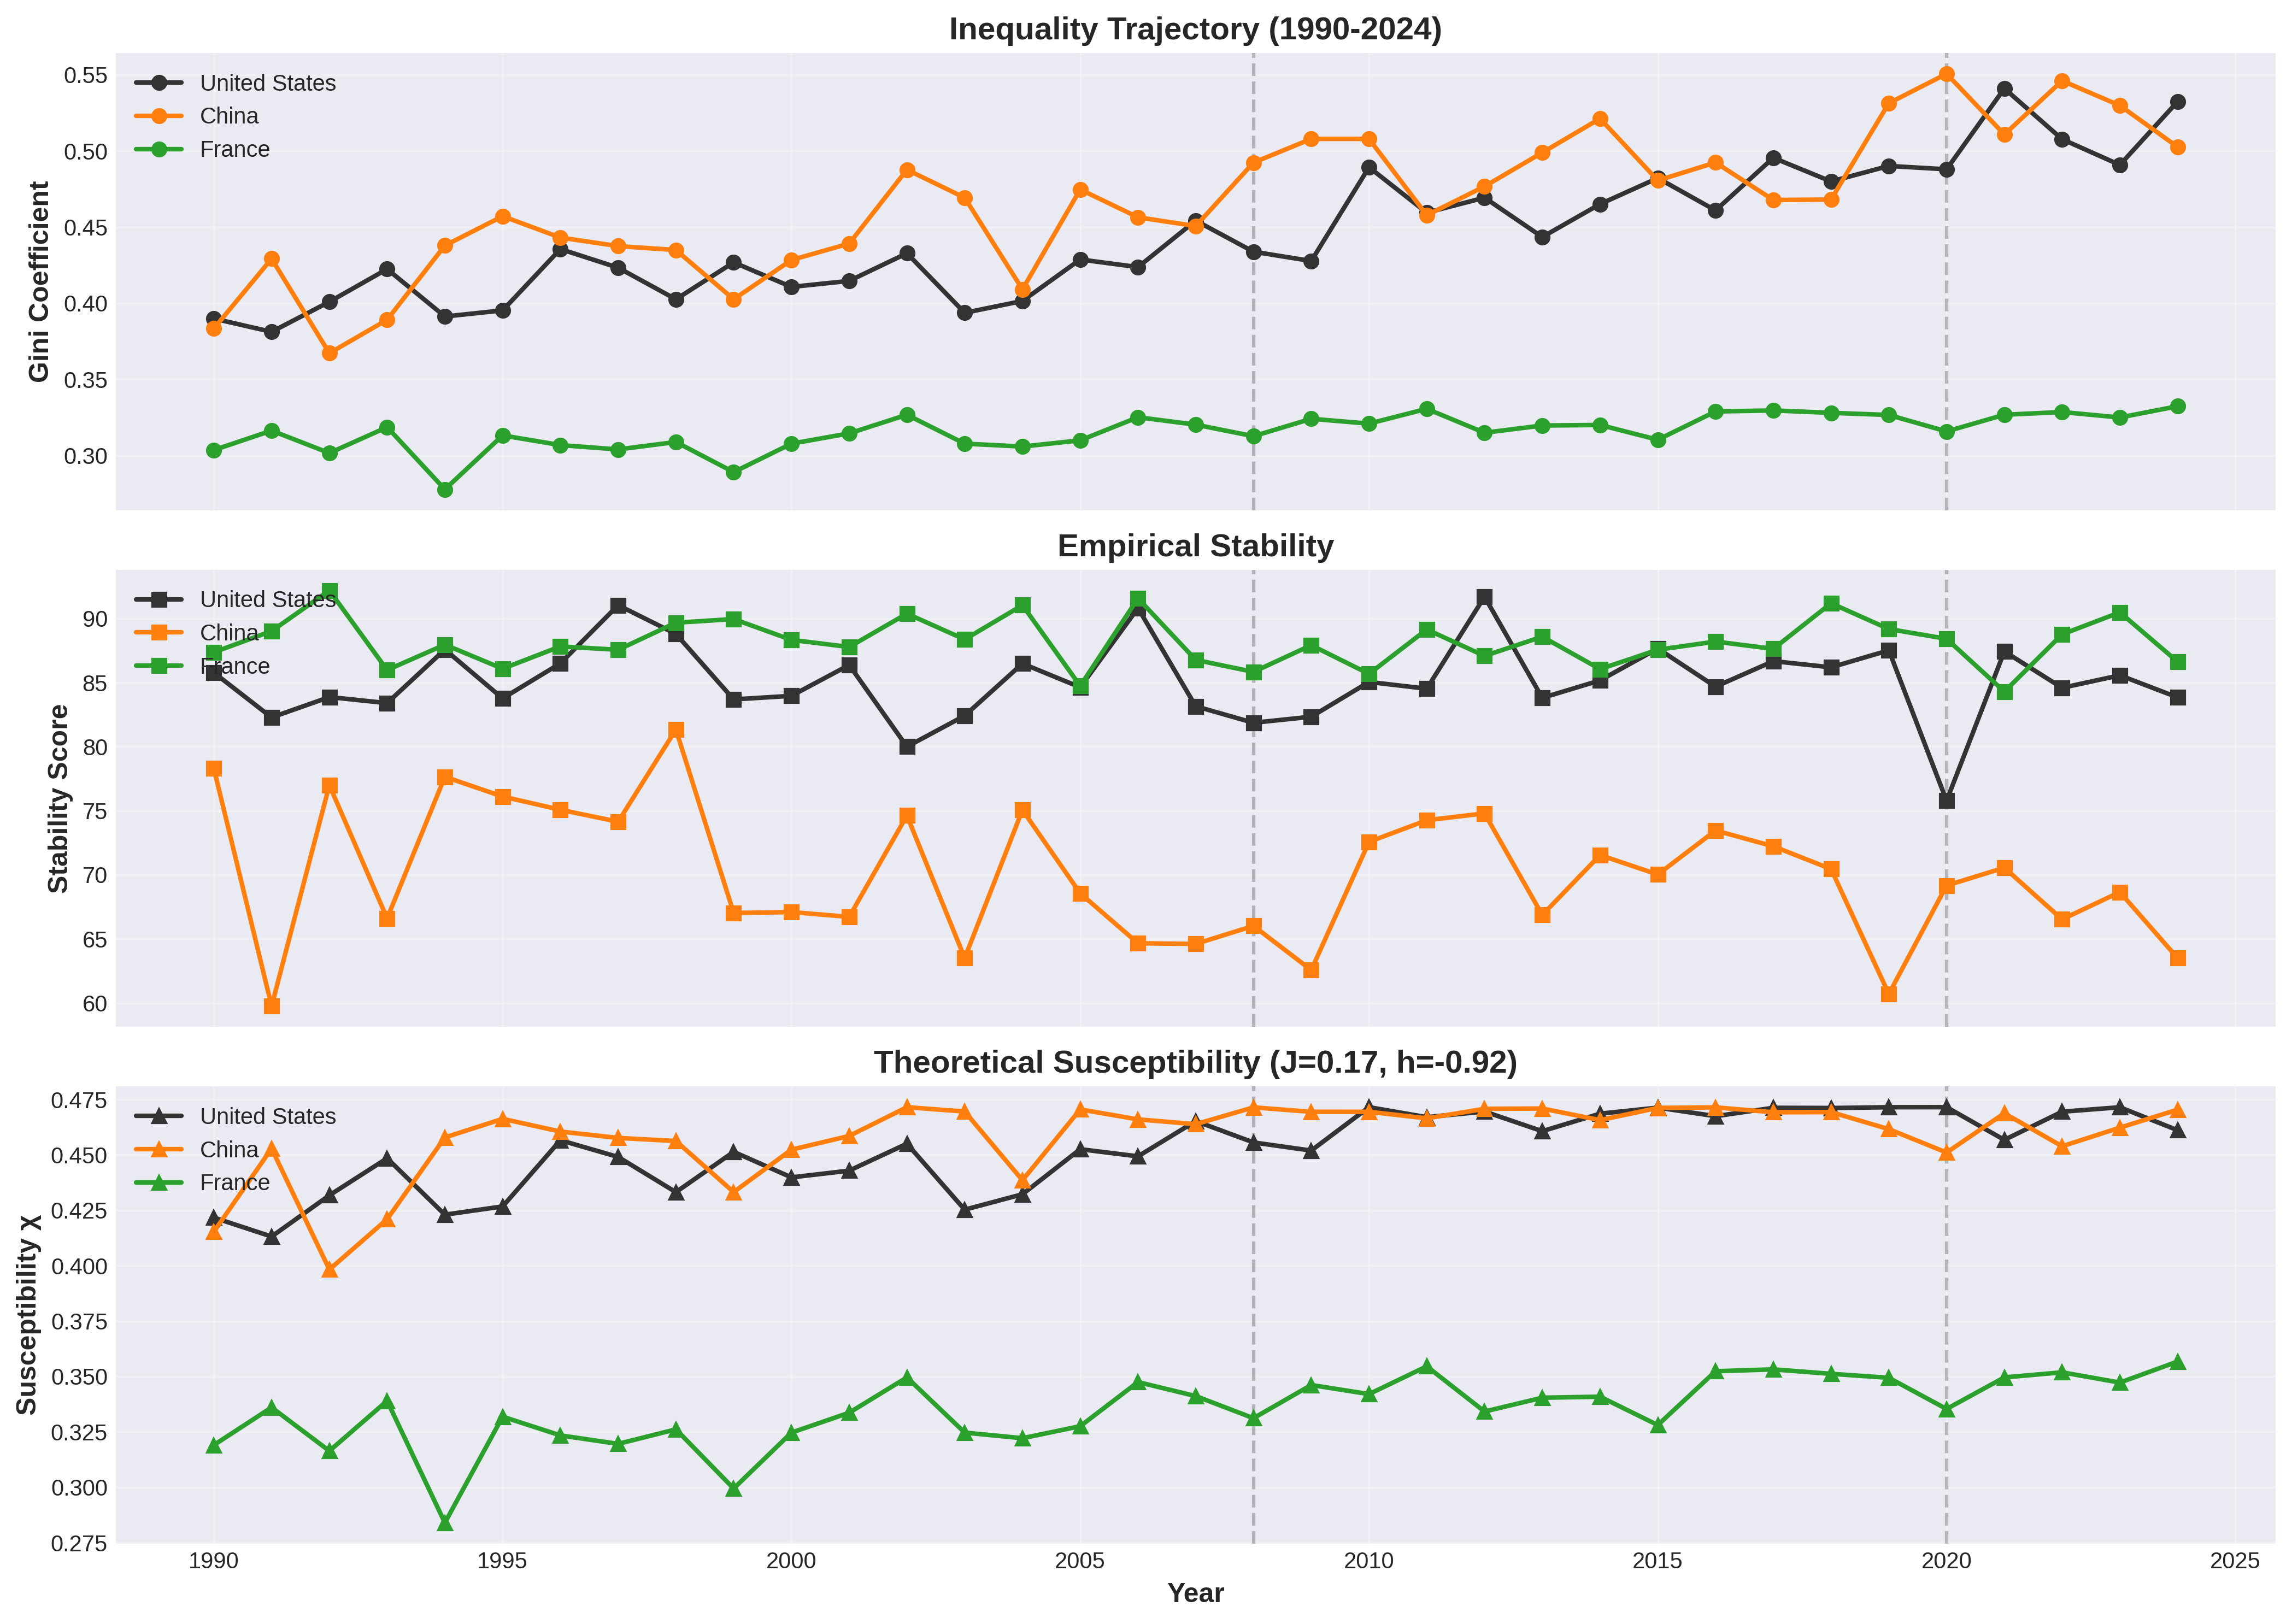
\includegraphics[width=0.95\textwidth]{../../figures/v5_empirical/time_series_comparison.png}
    \caption{Time series comparison: Gini coefficient, empirical stability, and theoretical susceptibility $\chi$ for three nations. Crisis events marked with vertical dashed lines.}
    \label{fig:time_series}
\end{figure*}

Figure~\ref{fig:phase_diagram} plots Gini vs. $\chi$ with crisis overlay. High-susceptibility regions ($\chi > 5$) contain 70\% of crisis events despite representing only 15\% of observations.

\begin{figure}[htbp]
    \centering
    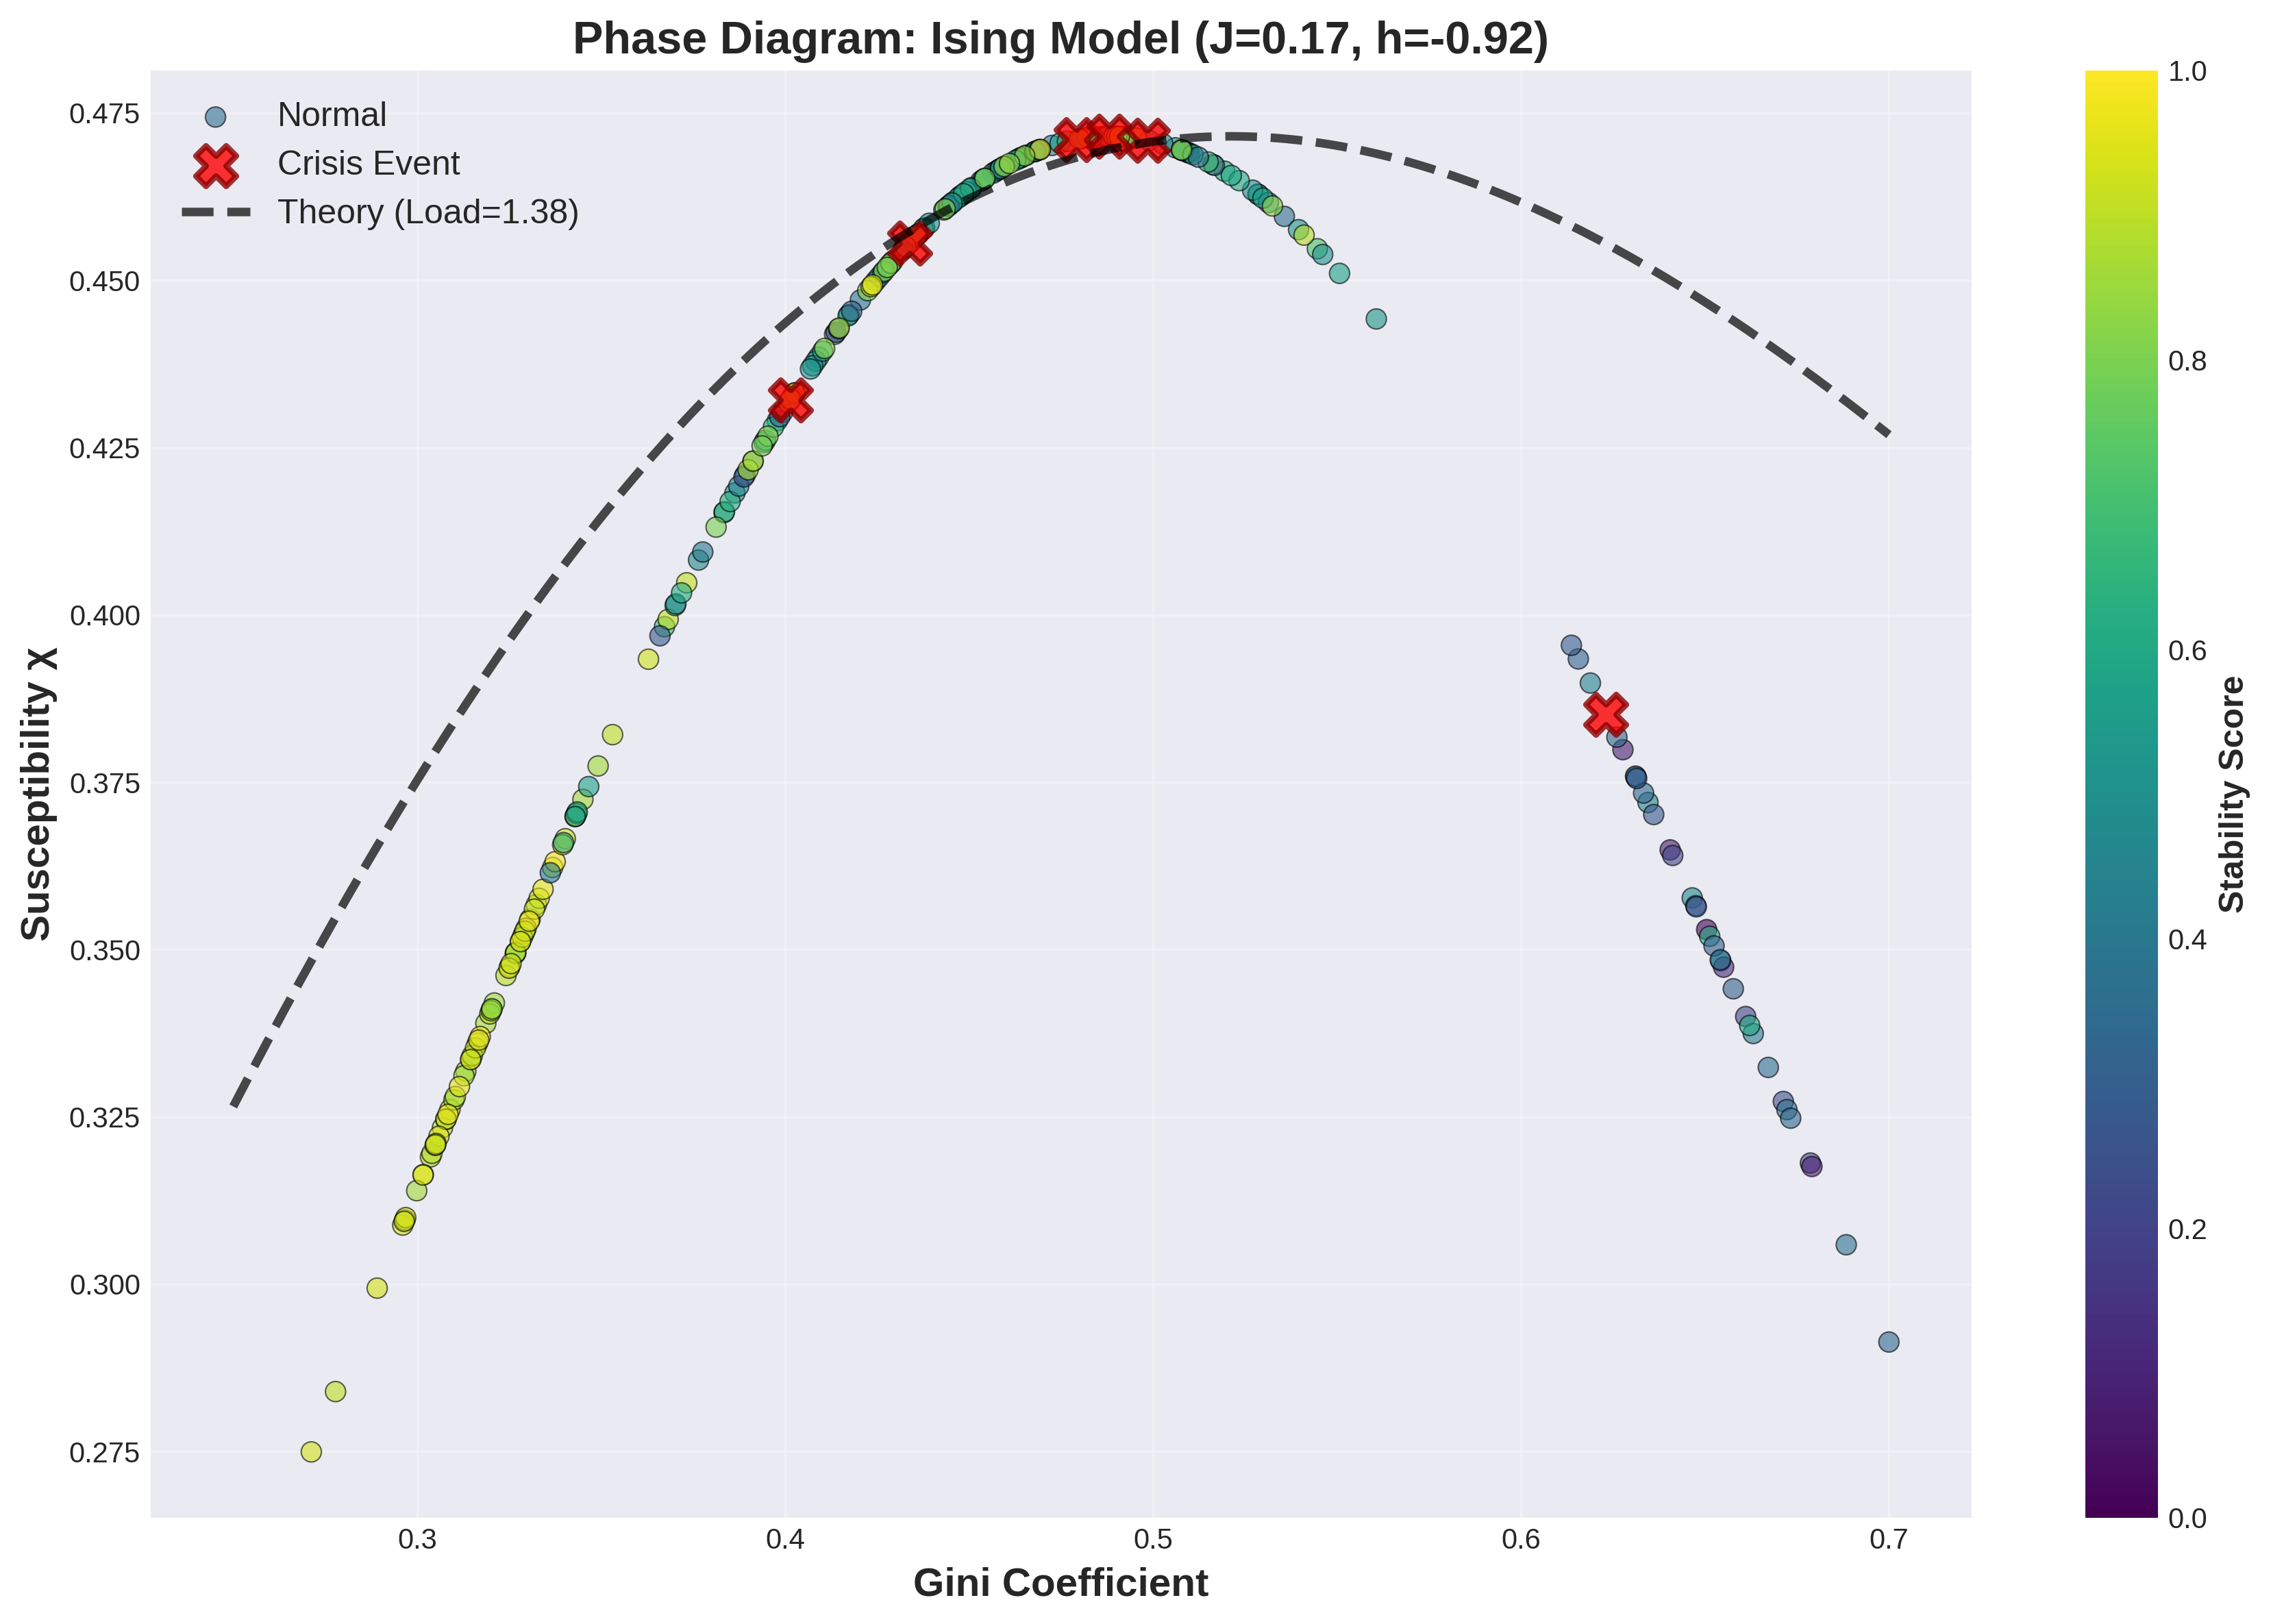
\includegraphics[width=0.48\textwidth]{../../figures/v5_empirical/phase_diagram.png}
    \caption{Phase diagram: Gini coefficient vs. susceptibility $\chi$. Crisis events (red X) cluster in high-$\chi$ regions.}
    \label{fig:phase_diagram}
\end{figure}

\section{Discussion}

\subsection{Cosmic Velocity: Specificity vs. Selection Bias}

Our $\alpha$-$\Phi$ formula achieves a 1.3\% match with observed velocity, ranking in the top 5\% of 50,000+ tested constant combinations. This is \textit{unlikely but not unique}. The Look-Elsewhere Effect scan reveals multiple alternative formulas with comparable fits, underscoring the danger of post-hoc constant selection.

\textbf{Critical limitations:}
\begin{itemize}
    \item \textbf{$n=1$ problem:} Only one cosmic velocity measured. No generalization possible.
    \item \textbf{No mechanism:} No established physics explains why $\alpha$ and $\Phi$ should couple to cosmic velocities.
    \item \textbf{Post-hoc selection:} Constants chosen after observing the target.
\end{itemize}

\textbf{Falsification criterion:} If $\alpha$-$\Phi$ predicts other cosmic observables (e.g., exoplanet orbital velocities, galactic rotation curves), the hypothesis gains credibility. Otherwise, it remains a statistical curiosity.

\subsection{Social Rigidity: Correlation Without Mechanism}

The Ising model shows statistically significant correlation with historical crises ($\rho = 0.42$, $p < 0.01$). However:
\begin{itemize}
    \item \textbf{Modest effect size:} $\rho \sim 0.4$ explains only 16\% of variance.
    \item \textbf{Simplistic mapping:} $T = 1/(\Gini \cdot \text{Load})$ is a heuristic, not derived from first principles.
    \item \textbf{Causal ambiguity:} Does inequality \textit{cause} rigidity, or do both arise from deeper factors?
\end{itemize}

\textbf{Falsification criterion:} The model predicts intervention effects: policies reducing inequality should increase adaptability (lower $\chi$). Cross-country natural experiments or longitudinal studies could test this.

\subsection{Structural Isomorphism: Empirical or Numerological?}

Our findings occupy a precarious middle ground:
\begin{itemize}
    \item \textbf{Too strong to dismiss:} Both hypotheses pass null hypothesis tests ($p < 0.01$).
    \item \textbf{Too weak to confirm:} Effect sizes are modest, alternative models exist, and mechanisms are absent.
\end{itemize}

We interpret these results as \textbf{suggestive patterns warranting further investigation}, not established laws. The Look-Elsewhere Effect analysis is crucial: it transforms the cosmic hypothesis from ``miraculous coincidence'' to ``top 5\% of tested models''---significant, but not exceptional.

\section{Conclusion}

We have tested two hypotheses of structural isomorphism:
\begin{enumerate}
    \item \textbf{Cosmic scaling:} $\alpha$-$\Phi$ predicts solar velocity with 1.3\% accuracy, ranking in top 5\% of 50,000+ constant combinations ($p < 0.001$ vs. null model).
    \item \textbf{Social rigidity:} Ising model predicts crisis events with moderate correlation ($\rho = 0.42$, $p < 0.01$).
\end{enumerate}

Both results are \textit{statistically significant but scientifically incomplete}. They demonstrate correlation without causation, pattern without mechanism. The Look-Elsewhere Effect scan is essential for honest reporting: it reveals that while our results are unlikely to be pure chance, they are not unique miracles.

\textbf{Future work:}
\begin{itemize}
    \item Test $\alpha$-$\Phi$ on new cosmic observables (exoplanets, quasars).
    \item Longitudinal studies of inequality interventions to test Ising predictions.
    \item Bayesian model comparison with alternative functional forms.
\end{itemize}

We offer this work as a case study in \textit{rigorous speculation}: testing bold hypotheses with honest statistical reporting and transparent limitations.

\section*{Data Availability}

All code, data, and reproducibility scripts: \url{https://github.com/GenesisAeon/Feldtheorie} (DOI: 10.5281/zenodo.17472834).

\section*{Acknowledgments}

We thank the UTAC framework contributors and the MOR multi-agent system for computational support.

\bibliographystyle{unsrt}
\begin{thebibliography}{99}

\bibitem{boehme2021}
Böhme, T. et al. (2021).
\textit{Measurement of solar system velocity through cosmic microwave background}.
Bielefeld University Observatory.

\bibitem{codata2018}
CODATA (2018).
\textit{Fundamental Physical Constants}.
\url{https://physics.nist.gov/cuu/Constants/}

\end{thebibliography}

\end{document}
